% DCL de la caja empujada a velocidad constante (DIAG-06: Fricción).
\documentclass[tikz,border=3pt]{standalone}
\usetikzlibrary{arrows.meta}
\begin{document}
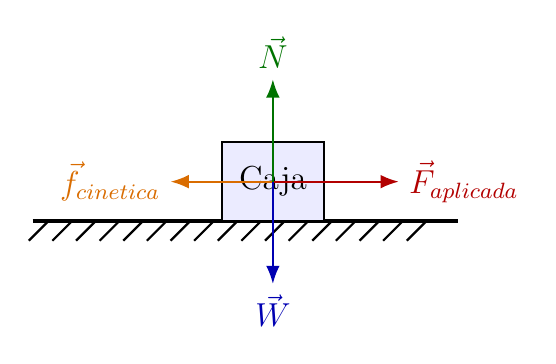
\begin{tikzpicture}[>=Latex, thick, font=\large]
  \draw[line width=1.2pt] (-2.4,0) -- (3,0);
  \foreach \x in {-2.2,-1.9,...,2.8} \draw (\x,0) -- (\x-0.25,-0.25);

  \draw[fill=blue!8] (0,0) rectangle (1.3,1);
  \node at (0.65,0.5) {Caja};
  \coordinate (centro) at (0.65,0.5);

  \draw[->, red!70!black] (centro) -- ++(1.6,0) node[right] {$\vec{F}_{aplicada}$};
  \draw[->, orange!85!black] (centro) -- ++(-1.3,0) node[left] {$\vec{f}_{cinetica}$};
  \draw[->, green!45!black] (centro) -- ++(0,1.3) node[above] {$\vec{N}$};
  \draw[->, blue!70!black] (centro) -- ++(0,-1.3) node[below] {$\vec{W}$};
\end{tikzpicture}
\end{document}
